\section{1. Introduction}

Early research in second language acquisition assumed that language could only be acquired through language-specific learning mechanisms (i.e., Universal Grammar \parencite{chomsky1965}). In this view, language learning was seen as entirely distinct from the processes described in general learning theory, with no interaction between the two. This assumption has led to a division between two fields that are fundamentally interested in the same process, yet remain largely disconnected — general learning theory and second language acquisition. This divide results in at least two fundamental issues: 1) the complexity of second language learning has not been sufficiently examined by the general learning literature, and 2) second language acquisition research has not taken full advantage of the extensive toolkit developed within general learning theory. Recently, this separation has been called into question, as general learning theory now posits that domain-general mechanisms can and do account for language acquisition throughout a person’s lifetime \cite[e.g.,][]{nixon2020mice}.

In the current study, we begin to bridge the gap between SLA and general learning theory by examining second language speech learning at and below the word level. We do this in two ways, we begin with a close replication of Nixon’s (2020) study on the general learning mechanisms that underpin Southern Min tone-word learning, while also extending the general learning paradigm to the learning of Japanese vowels and Mandarin fricatives. This replication of Southern Min and cross-language extension to Mandarin and Japanese contribute not only to the need for close replication \parencite{Marsden_2018}, but also stands as a test of generalizability for using general learning theory in SLA. Secondly, in an exploratory analysis, we methodologically adapt \textcite{nixon2020mice}'s original study design so that we can operationalize eye-fixations as a measure to account for surprisal in learning. That is, we go beyond behavioral accuracy during testing and dive into the mechanisms which drive learning by examining eye-fixations during training. 

\subsection{Speech Learning in SLA}

Learning to perceive lower-level speech contrasts in a second language is a central challenge in SLA. Whereas first language speakers have highly developed skills for distinguishing fined grained phonetic differences of their L1 (e.g., distinguishing \textit{surprise} and \textit{supplies}), unsuccessful second language speech perception (e.g., perceiving /r/ and /l/ the same for L1 Japanese learners of English) creates unnecessary competition during lexical selection. This competition only increases the already multi-faceted challenge of successful communication in a second language. In all languages, distinguishing word meanings requires that learners are able to distinguish sub-word segmental differences (i.e., consonants and vowels) with many languages requiring an additional sensitivity to suprasegmental differences (e.g., tone, pitch-accent, stress). In this way, for the second language learner, each language presents its own unique set of challenges, and the degree of difficulty learners experience often depends on the nature of the L2 contrasts relative to their L1 speech contrasts and lexicon \parencite{Flege1995,Best1995,BestTyler2007,vanLeussenEscudero2015}. 

In the same way that L1 speakers have learned to distinguish meaningful features in their first language, L2 learners struggle to distinguish between sounds that are not meaningful in their L1. The majority of second language speech research has focused on the learning of segmental contrasts. One of the most well known and prolific examples is Japanese speakers frequent struggles with English /r/ and /l/ sounds even after years of learning \parencite{Brown2000}. However, Japanese speakers are not alone. For example: Mandarin learners struggle with English fricatives (\textipa{/v/, /\texttheta/, /\dh/}) \cite{Wiener2022} and English speakers struggle with Arabic pharyngeal \cite{Burnham2013} and Spanish /b/ and /p/ \cite{Nagle2022}. Even harder some languages have three way contrasts (e.g., Korean's tense-lax-aspirated stop contrasts), which L2 learners continue to have difficulty with even in advanced study \cite{Kim2023}. 

Vowels too can be difficult. 

While less studied, suprasegmental learning in the second language poses its own challenges for second language learners. Learners from non-tone language backgrounds struggle to discriminate or identify tones. While training is consistently found to improve identification 

To explain the challenge of second language speech learning, several models of L2 speech perception and production have been developed. The Perceptual Assimilation Model (PAM), explains that the degree of difficulty in perceiving L2 sounds depends on how they are assimilated into the learner’s L1 categories. For example, when two L2 sounds map onto the same L1 category (e.g., English /r/ and /l/), learners struggle more to differentiate them, while contrasts that map onto two distinct L1 categories are easier to learn. Similarly, the Speech Learning Model (SLM) emphasizes that learners’ ability to acquire new phonetic categories in an L2 is influenced by the interaction between the L1 and L2 phonetic systems. Yet, both models are limited by only describing where such difficulties may arise not in trying to understand the mechanisms that aid learning or improve learner's abilities to perceive these difference in order to improve language skills and communication.

The complexity of speech learning is compounded by the continuous and unconscious nature of speech processing, which involves dynamically varying acoustic cues (e.g., pitch, duration, and VOT). Whether learning to perceive a small boundary shift in a cue (e.g., VOT for English /b/, Spanish /b/, and Mandarin /b/) or learning entirely new dimensions of speech (e.g., Lexical stress or tone), learners must adapt to these cues to make meaning in their L2.

\subsection{General Learning Mechanisms}

Language learning, particularly the acquisition of speech contrasts, can be understood through two complementary learning mechanisms: statistical learning and error-driven learning. Statistical learning allows learners to detect regularities in the speech input, forming and adjusting categories based on frequency and distribution. Yet, for second language learners, getting enough input to overcome their L1 speech categories is not only difficult but may be impossible, as even advanced learners continue to struggle with certain features. For example, advanced Mandarin learners persistently face challenges in mastering tonal distinctions despite extensive training (Pelzl et al., 2021). This persistent difficulty suggests that learners need more than just repeated exposure to L2 input. Instead, more adaptive mechanisms are required. One possible learning mechanism is error-driven learning, which utilizes prediction-error or surprisal to drive adjustments in learners' speech categories. When the L2 input deviates from the learner's expectations, based on their L1 categories, this mismatch provides an opportunity for learning. For example, when a Mandarin learner first comes across the word -(Korean) they are likely to think it means Chinese. This is because they know the word for Chinese  and it is segmentally identical to Korean with only 1 tone being different. The discrepancy between expectation and experience creates a prediction error that facilitates learning. This mechanism can help learners move beyond the limitations of their L1 categories by focusing on moments of uncertainty between what they are expecting and what they hear.

Generally, models of statistical Learning posit that learners track the frequency and co-occurrence of acoustic cues. The basic assumption is that learners accumulate knowledge by being exposed to input, where frequently co-occuring sound meaning relationships guide learning. For example, in this model, learners would gradually learn phonetic contrasts by recognizing how often particular sounds or features occur in the speech they are exposed to. The underlying principle of this model is that frequent exposure leads to stronger mental representations of these sounds, allowing learners to form categories based on this accumulated evidence. 

Error-Driven Learning, by contrast, focuses on the role of surprisal, or prediction error, in shaping learning. In this framework, learners make predictions about incoming linguistic input based on their existing knowledge, and when those predictions are violated, learning occurs. Learning, then, is not simply about exposure or frequency but is driven by the degree of mismatch between expectation and reality. When a learner encounters a speech cue that does not align with their prediction (e.g., misidentifying a tone/vowel/fricative), this generates prediction error, which prompts the learner to adjust their internal models to better match the input. 

While the difference between statistical learning and error-driven learning may initially seem subtle, it has profound implications for how learners process language. On the surface, both mechanisms aim to explain how learners acquire speech contrasts through exposure to acoustic cues. However, statistical learning emphasizes the accumulation of associations through repeated exposure, whereas error-driven learning relies on the dynamic process of making predictions and adjusting based on errors. One critical distinction is that prediction requires time— learners need to process cues and anticipate outcomes before the outcome is known. In contrast, association can occur without a temporal structure, as it simply involves linking two events that co-occur, regardless of their order.

Moreover, these mechanisms diverge significantly when it comes to the role of positive evidence vs. unlearning. Statistical learning suggests that learners rely on the positive co-occurrence of cues and outcomes, gradually building an understanding of the relationship between the two based on how often they appear together. In this framework, learning is about reinforcing these connections through repeated exposure. However, error-driven learning emphasizes the importance of unlearning irrelevant cues—when a cue does not reliably predict the correct outcome, learners must downweight its influence. This process of unlearning allows learners to focus on the more discriminative cues, sharpening their ability to accurately predict outcomes in the future.

\subsection{Nixon’s Study on Error-Driven Learning}

Nixon (2020), the study replicated here, provides a compelling case for error-driven learning in speech sound learning. Her study examine the learning of 6 Southern Min words. 

. In this study, Nixon demonstrated that learners update their internal models of speech not solely by tracking the frequency of speech cues but through feedback-driven adjustments when their predictions about speech sounds fail. The study revealed that cue competition and unlearning play a central role in shaping speech sound acquisition, challenging purely statistical models that emphasize passive exposure.

Nixon's findings highlight the critical role of prediction error in L2 speech learning, especially in tonal contrasts, where subtle acoustic differences are critical for meaning. By demonstrating that learners adjust their phonological representations based on feedback from failed predictions, Nixon's study supports the notion that error-driven learning is central to the acquisition of new phonological categories in a second language. This aligns with broader theories of general learning mechanisms and offers insights into how L2 learners navigate the challenges of acquiring complex phonological contrasts.

discriminative and non-discriminative presentation orders

\begin{figure}[H]
  \centering
  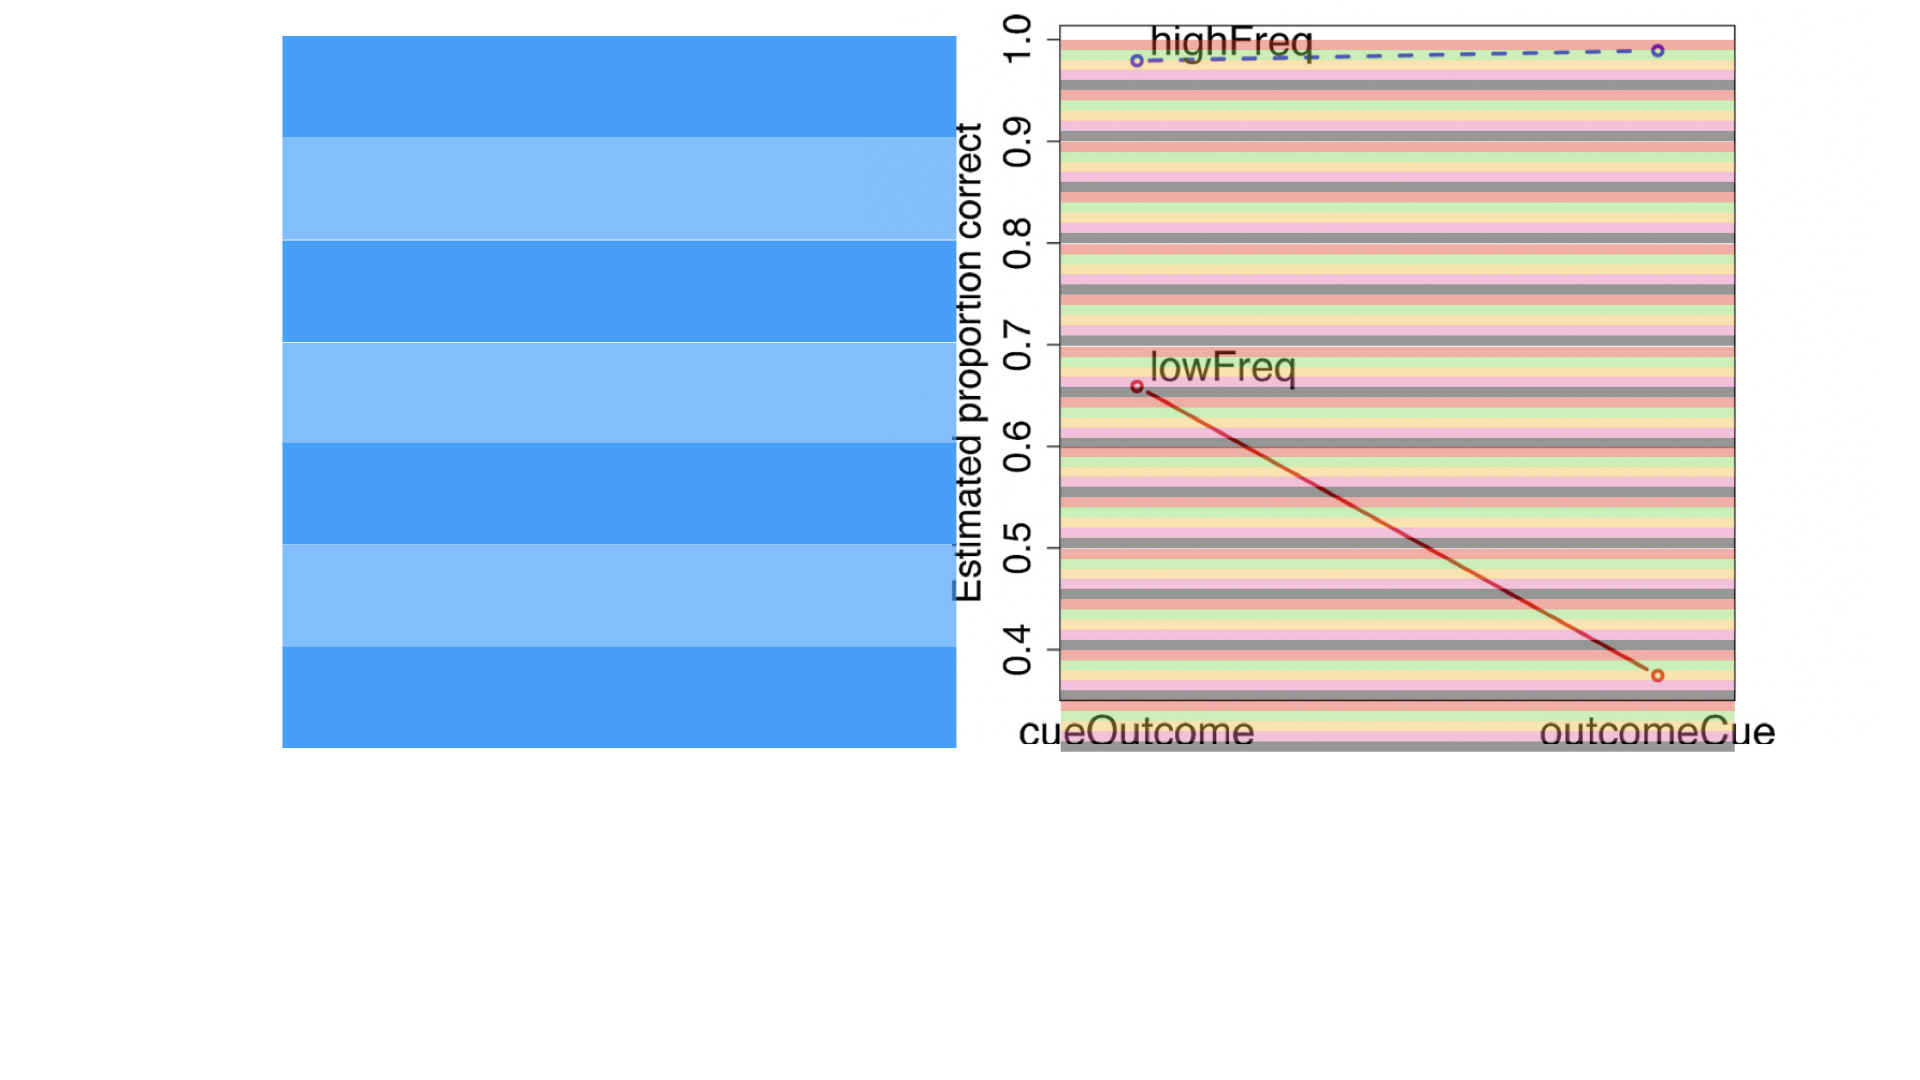
\includegraphics[width=1\linewidth]{visualizations/visualizations/visualizations.005.jpeg}
  \caption{nixon stim}
  \label{fig:nixon_stim}
\end{figure}



\subsection{The Current Study: Extending Nixon (2020)}

In the current study, we replicate Nixon (2020) study on Southern Min tone learning, and extend the experimental design to include two new languages: Mandarin and Japanese. In the following experiments our primary goal is to test the predictions of statistacl and error-driven learning in speech acquisition by examining lower-level contrasts in three areas: suprasegmental (Southern Min tone), segmental (Japanese vowel length), and segmental (Mandarin fricatives).  Additionally, by including Japanese and Mandarin contrasts, we test the generalizability of error-driven learning mechanisms across different phonetic domains and languages.

In an exploratory analysis of the training data, we extend the methodology by incorporating eye-tracking data, operationalizing eye-fixations as an indicator of prediction errors. This allows us to move beyond behavioral accuracy and directly examine how learners’ real-time processing of speech is influenced by prediction errors. By tracking learners’ eye movements during training, we can gain a more nuanced understanding of how learners adapt to new phonological contrasts through surprisal in learning.

\subsubsection{Mandarin Fricatives/africates and Japanese Vowel Duration}

Mandarin presents a unique phonological structure, particularly with the *zh-j* fricative contrast, which are differentiated by higher and lower amplitude. Learners must rely on fine distinctions in place of articulation to correctly identify these sounds, making it an ideal case for studying prediction error. Mandarin fricatives and affricates have three places of articulation. In the current study, we explore the learning of the retroflexive and Alveolopalatal. 

\textbf{IPA for the sound in "judge":} \textipa{[dZ]}

\textbf{IPA for the sound in "zhang" (Mandarin):} \textipa{[tS\super{r}]}

\textbf{IPA for the sound in "jiang" (Mandarin):} \textipa{[tC]}


This is a postalveolar sound, produced with the tip of the tongue curled back toward the hard palate just behind the alveolar ridge
This is a sound produced with the tongue positioned near the hard palate, but further forward than retroflex sounds

In Japanese, vowel duration plays a critical role in lexical meaning, as exemplified by words like *kuti* (mouth) and *kuuti* (air). The ability to distinguish between short and long vowels is crucial for accurate speech perception and production. Examining how prediction error influences the learning of vowel length distinctions provides insight into how learners adjust their perception of temporal features in speech, further expanding our understanding of error-driven learning in vocalic contrasts.

\subsection{Rationale for the Eye-Tracking Extension}

In addition to replicating the unlearning experiment across Mandarin and Japanese, we incorporate an eye-tracking extension to operationalize prediction errors during training. Eye-tracking allows us to observe how learners' gaze patterns reflect their real-time adjustments to prediction errors. By tracking visual attention during speech tasks, we can measure the immediate feedback-driven learning process and observe how prediction errors are corrected over time.

\subsection{Contributions to the Field}

This study builds on Nixon's foundational work, extending error-driven learning to consonants and vowels in Mandarin and Japanese. By focusing on fricatives and vowel duration, this research deepens our understanding of how prediction errors function across different phonetic dimensions. The addition of eye-tracking further enhances our ability to capture the dynamic process of prediction error correction, offering a novel perspective on real-time learning in speech acquisition.

\section{Research Questions and Hypotheses}

\subsection{Research Questions}

\begin{itemize}
    \item  To what extent does discriminative and non-discriminative learning order affect the learning of Japanese words with contrastive vowel length.
    \item To what extent does discriminative and non-discriminative learning order affect the learning of Mandarin words with contrastive fricatives.
    \item To what extent does discriminative and non-discriminative learning order affect the learning of Southern Min words words with contrastive tones.
   \item To what extent can eye-fixations be used as a measure of prediction-error during training to account for learning outcomes.
\end{itemize}

\subsection{Hypotheses}

\begin{itemize}
    \item High frequency words will be learned across all languages. 
    \item Low frequency words will be learned less well across all languages assuming that high frequency words are learned.
    \item Low frequency words will be learned better in the discriminative learning order because of higher prediction error.
    \item Prediction-error (as estimated through eye-fixations) will be highest in discrimitive order condition. 
    \item Prediction-error (as estimated through eye-fixations) will be highest in low frequency items.
\end{itemize}